\documentclass[a4paper,12pt]{report}
\usepackage[utf8]{inputenc}
\usepackage[francais]{babel}
\usepackage[T1]{fontenc}
\usepackage{graphicx}
\usepackage{listingsutf8}
\usepackage[colorlinks,urlcolor=blue]{hyperref} %hyperlinks
\usepackage[nottoc,notlot,notlof]{tocbibind} %To bind the table of contents to the bibligoraphy
\usepackage{../../../packages/tikz-uml} %UML elements

\lstset{
    language=SQL,
    commentstyle=\color{blue!80}\upshape,
    keywordstyle=\color{red!60},
    basicstyle=\ttfamily\small,
    backgroundcolor=\color{gray!10}, %code with gray background
    rulecolor=\color{black!30},
    numberstyle=\footnotesize, %line numbers for the code
    numbers=left, %numbers to the left
    breaklines=true,
    breakatwhitespace=true,
    frame=single,
    framextopmargin=2pt,
    framexbottommargin=2pt,
    captionpos=b,
    inputencoding=utf8,
    extendedchars=true, %to extend the default charset
    literate={á}{{\'a}}1 {é}{{\'e}}1 {í}{{\'i}}1 {ó}{{\'o}}1 {ú}{{\'u}}1 {Á}{{\'A}}1 {É}{{\'E}}1 {Í}{{\'I}}1 {Ó}{{\'O}}1 {Ú}{{\'U}}1 {à}{{\`a}}1 {è}{{\`e}}1 {ì}{{\`i}}1 {ò}{{\`o}}1 {ù}{{\`u}}1 {À}{{\`A}}1 {È}{{\'E}}1 {Ì}{{\`I}}1 {Ò}{{\`O}}1 {Ù}{{\`U}}1 {ä}{{\"a}}1 {ë}{{\"e}}1 {ï}{{\"i}}1 {ö}{{\"o}}1 {ü}{{\"u}}1 {Ä}{{\"A}}1 {Ë}{{\"E}}1 {Ï}{{\"I}}1 {Ö}{{\"O}}1 {Ü}{{\"U}}1 {â}{{\^a}}1 {ê}{{\^e}}1 {î}{{\^i}}1 {ô}{{\^o}}1 {û}{{\^u}}1 {Â}{{\^A}}1 {Ê}{{\^E}}1 {Î}{{\^I}}1 {Ô}{{\^O}}1 {Û}{{\^U}}1
    {œ}{{\oe}}1 {Œ}{{\OE}}1 {æ}{{\ae}}1 {Æ}{{\AE}}1 {ß}{{\ss}}1
    {ű}{{\H{u}}}1 {Ű}{{\H{U}}}1 {ő}{{\H{o}}}1 {Ő}{{\H{O}}}1 {ç}{{\c c}}1 {Ç}{{\c C}}1 {ø}{{\o}}1 {å}{{\r a}}1 {Å}{{\r A}}1 {€}{{\euro}}1 {£}{{\pounds}}1 {«}{{\guillemotleft}}1 {»}{{\guillemotright}}1 {ñ}{{\~n}}1 {Ñ}{{\~N}}1 {¿}{{?`}}1
}

\begin{document}
%----------------------------------------------------------------------------------------
%   TITLE PAGE
%----------------------------------------------------------------------------------------
\begin{titlepage}
\newcommand{\HRule}{\rule{\linewidth}{0.5mm}} % Defines a new command for the horizontal lines
\center
%----------------------------------------------------------------------------------------
%   LOGOS SECTION
%----------------------------------------------------------------------------------------

\includegraphics[scale=0.5]{images/umLogo.png} % Université de Montpellier Logo
\hspace{\fill}

\includegraphics[scale=0.25]{images/fdsLogo.jpg} % Faculté de Sciences Logo
%----------------------------------------------------------------------------------------
%   HEADING SECTIONS
%----------------------------------------------------------------------------------------
\textsc{\LARGE M1 Informatique AIGLE}\\[1cm]
\textsc{\Large \textbf{HMIN122M}}\\[0.25cm]
\textsc{\large Mini-Projet : entrepôts de données}\\[0.8cm]
%----------------------------------------------------------------------------------------
%   TITLE SECTION
%----------------------------------------------------------------------------------------
\HRule \\[0.4cm]
{ \huge \bfseries Rapport}\\[0.4cm]
\HRule \\[0.8cm]
%----------------------------------------------------------------------------------------
%   AUTHORS SECTION
%----------------------------------------------------------------------------------------
\begin{minipage}{\textwidth}
\centering \huge
Bachar \textsc{Rima}\\ % Student
Joseph \textsc{Saba}\\ % Student
Tasnim \textsc{Shaqura Muhammad}\\ % Student
Jérémy \textsc{Bourgin} % Student
\end{minipage} \\[0.8cm]
%----------------------------------------------------------------------------------------
%   DATE SECTION
%----------------------------------------------------------------------------------------
{\large \today}\\[1cm]
\hspace{\fill}
\vfill % Fill the rest of the page with whitespace
\end{titlepage}

\pagestyle{plain}

{
  \hypersetup{linkcolor=black}
  \tableofcontents
}

\newpage

\chapter{Introduction}
\section{Problématiques}
Dans le cadre du mini-projet du module \textbf{HMIN122M}, nous avons décidé de modéliser un entrepôt de données pour le réseau de transport publique de Montpellier, \textit{tam-voyages}. Pour ce faire, nous avons proposé des \textit{data marts} formant le \textit{data warehouse}, et permettant de réaliser des requêtes analytiques sur un ensemble important de données. Cette modélisation permettra ainsi de mettre en \oe{}uvre un outil d'analyse pour répondre aux problématiques suivantes :
\begin{enumerate}
  \item Comment peut-on tirer partie de la fréquentation des véhicules en se basant sur la circulation du réseau\footnote{en particulier en examinant les lignes de tramway et les bus} afin d'améliorer la qualité de service (e.g. \textit{nombre de véhicules à envoyer sur une ligne pendant une certaine période de la journée})?
  \item Comment peut-on suivre l'évolution et la maintenance des matériaux de manière à réduire les dépenses associées ?
\end{enumerate}

Pour répondre à ces problématiques, nous énumérons les actions et opérations effectuées par \textit{tam-voyages}. Ensuite, nous choisirons celles qui paraissent les plus pertinentes en termes de données intégrées et flexibilité des critères d'analyse.

\section{Actions et opérations}
Les actions/opérations effectuées par \textit{tam-voyages} considérées :
\begin{itemize}
  \item les voyages.
  \item la maintenance de véhicules.
  \item les ventes de tickets et les abonnements.
  \item les amendes.
\end{itemize}

\section{Exemples de requêtes analytiques possibles}
\begin{enumerate}
  \item exemples de requêtes analytiques pour l'action \og voyages \fg :
  \begin{itemize}
    \item \texttt{le nombre de voyages par bus, utilisant des tickets pour le mois de juillet.}
    \item \texttt{le nombre de voyageurs abonnés par ligne pour chaque voyage pour les deux derniers mois.}
    \item \texttt{l'arrêt le plus fréquenté par ligne.}
  \end{itemize}
  \item exemples de requêtes analytiques pour l'action \og maintenance \fg :
  \begin{itemize}
    \item \texttt{le coût total de maintenance de chaque véhicule.}
    \item \texttt{le nombre total de maintenances effectuées sur les bus par employé pour l'année 2018.}
    \item \texttt{le nombre total de maintenances effectuées par véhicule pour les 6 dernier mois.}
  \end{itemize}
  \item exemples de requêtes analytiques pour l'action \og ventes \fg :
  \begin{itemize}
    \item \texttt{le nombre d'abonnés ayant plus que 26 ans pour le mois d'août 2018.}
    \item \texttt{le nombre d'abonnés par date de naissance pour l'année 2018.}
    \item \texttt{les types d'abonnement les plus fréquents pour l'année 2018.}
  \end{itemize}
  \item exemples de requêtes analytiques pour l'action \og amendes \fg :
  \begin{itemize}
    \item \texttt{les lignes qui ont générées le plus d'amendes pour les deux derniers mois.}
    \item \texttt{les lignes les plus contrôllées de la semaine dernière.}
    \item \texttt{le nombre des abonnés qui ont reçu des amendes par ligne, l'avant-midi.}
    \item \texttt{la somme total d'amendes rapportée par type de voyageur par ligne pour le dernier mois.}
  \end{itemize}
\end{enumerate}

\chapter{Modélisation}
\section{Choix des actions à modéliser}
Les actions considérées, par ordre d'importance:
\begin{enumerate}
  \item \og voyages \fg.
  \item \og ventes \fg.
  \item \og maintenance \fg.
  \item \og amendes \fg.
\end{enumerate}

Les actions les plus pertinentes à analyser vis-à-vis les problématiques avancées sont \og voyages \fg et \og maintenance \fg qu'on traitera de la manière suivante :
\begin{description}
  \item [voyages :] modèle en étoile détaillé.
  \item [maintenance :] modèle en étoile \textit{moins} détaillé, en particulier le modèle intitulé "\textit{record transaction}".
\end{description}

\section{Modélisation des voyages}
\begin{figure}[!ht]
  \centering
  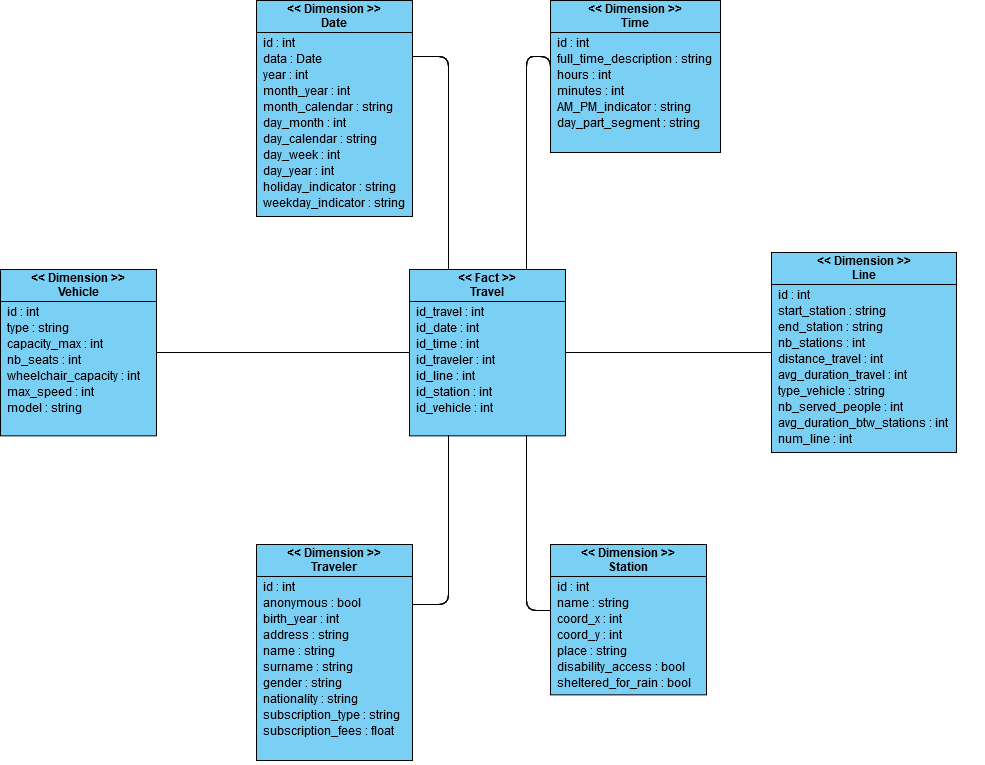
\includegraphics[scale=0.4]{images/voyages_datamart.png}
  \caption{modèle en étoile de l'action \og voyages \fg}
\end{figure}

\newpage

\subsection{Discussion}
\begin{itemize}
  \item un fait correspond à un voyage (\texttt{Travel}) effectué par un voyageur à un temps donné et une date donnée, en prenant un véhicule d'une ligne depuis un arrêt spécifié.
  \item chaque tuple dans la table \texttt{Vehicle} désigne un véhicule possédé par la société.
  \item chaque tuple dans la table \texttt{Ligne} désigne une itinéraire prise par une ligne. Autrement dit, la même ligne peut avoir plusieurs itinéraires différentes (\textit{e.g. la ligne 3 possède 4 itinéraires différentes})
  \item chaque tuple dans la table \texttt{Station} désigne une station desservie par un véhicule.
  \item la table \texttt{Traveler} est une dimension qui contient deux dimensions corrélées (les abonnés et le voyageur anonyme non abonné, utilisant un ticket) :
  \begin{enumerate}
    \item si le voyageur est \textbf{abonné}, alors on traite le tuple correspondant en tant qu'un \textbf{voyageur concret} dont les informations sont à notre disposition.
    \item sinon, tous les \textbf{voyageurs non abonnés} seront représentés par un seul tuple.
    \item cette décision de corrélation est utilisée pour éviter la normalisation et l'introduction d'une superclasse abstraite étendue par les classes désignant les voyageurs abonnés et non abonnés.
    \item nous utilisons ainsi l'attribut \textbf{anonymous} afin de distinguer les deux types de voyageurs. En effet, \textbf{anonymous} valera \textit{true} quand le voyageur est non abonné, sinon il valera \textit{false}.
    \item le tuple du \textbf{voyageur non abonné} contiendra ainsi des \textbf{valeurs nulles} pour les attributs décrivant un \textbf{voyageur abonné}.
  \end{enumerate}
\end{itemize}

La table des voyages n'admet aucune mesure; on se contentera d'utiliser les informations fournies par les dimensions qui suffiront largement pour analyser la fréquentation des différentes lignes et véhicules correspondant.

\subsubsection{Remarques}
\begin{itemize}
  \item l'attribut \textbf{id\_travel} de la table \texttt{Travel} est la clé primaire utilisée pour identifier un voyage (\textit{dimension dégénérée}).
  \item l'attribut \textbf{nb\_served\_people} de la table \texttt{Line} désigne le nombre de passagers désservis par la ligne.
  \item l'attribut \textbf{place} de la table \texttt{Station} désigne l'endroit où se trouve la station (\textit{e.g. avenue $X$, rue $Y$, $\dots$}).
  \item l'attribut \textbf{wheelchair\_capacity} de la table \texttt{Vehicle} désigne la capacité théorique maximale de personnes handicappées et de leurs fauteuils roulants.
\end{itemize}

\section{Modélisation des maintenances}
\begin{figure}[!ht]
  \centering
  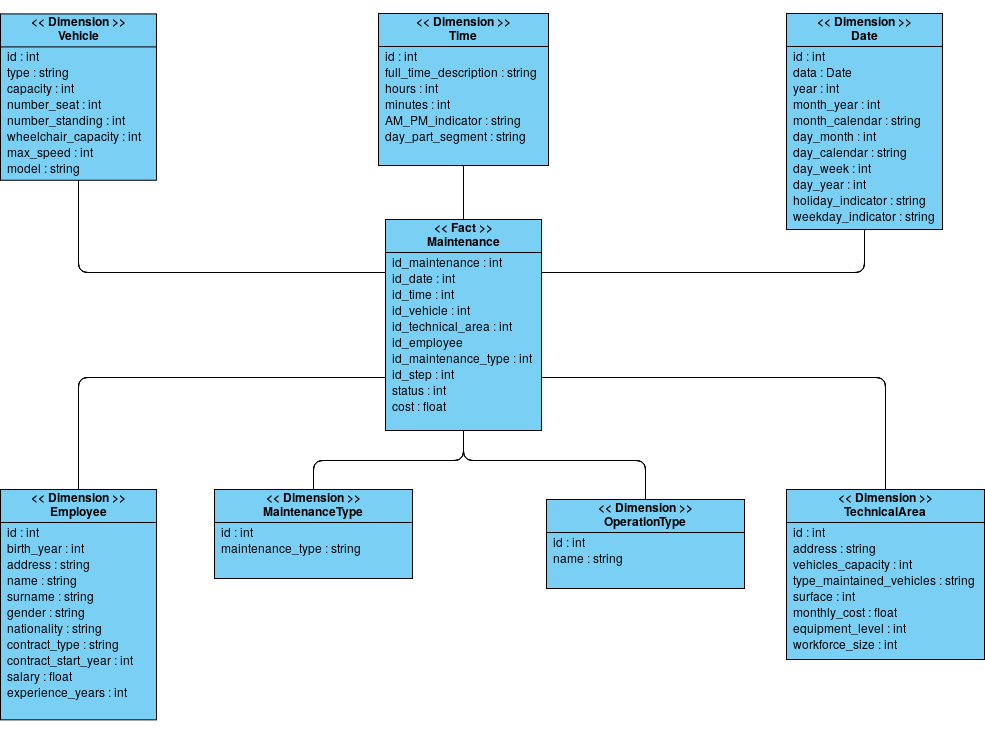
\includegraphics[scale=0.4]{images/maintenance_datamart.png}
  \caption{modèle en étoile de l'action \og maintenance \fg}
\end{figure}

\subsection{Discussion}
\begin{itemize}
  \item un fait désigne l'état d'une opération lors de la maintenance \texttt{Maintenance} d'un véhicule (\textit{i.e. le grain choisi pour la maintenance est la transaction}).
  \item chaque tuple dans la table \texttt{Employee} désigne un employé chez \textit{tam-voyages}.
  \item chaque tuple dans la table \texttt{TechnicalArea} désigne un dépôt utilisé par \textit{tam-voyages} pour maintenir des véhicules.
  \item chaque tuple dans la table \texttt{MaintenanceType} désigne un type de maintenance effectuée (\textit{e.g. changement de roues, maintenance du moteur, $\dots$})
  \item chaque tuple dans la table \texttt{OperationType} désigne une opération faite lors de la maintenance d'un véhicule (\textit{i.e. type de transaction effectuée}). Ne connaissant pas les détails des opérations effectuées par \textit{tam-voyages}, nous proposons les opérations suivantes :
  \begin{enumerate}
    \item conduire le véhicule concerné vers un dépôt de maintenance (\textit{i.e. début de la maintenance})
    \item allouer un garage pour la maintenance du véhicule.
    \item attribuer la maintenance du véhicule à un spécialiste.
    \item éventuellement attendre l'acquisition de ressources nécessaires à la maintenance du véhicule.
    \item mise en marche du véhicule dans le réseau après sa maintenance (\textit{i.e. fin de la maintenance})
  \end{enumerate}
\end{itemize}

Les mesures de la table \texttt{Maintenance} sont :
\begin{itemize}
  \item \texttt{cost} : mesure additive désignant le coût de maintenance d'un véhicule pour une transaction donnée.
\end{itemize}

\subsubsection{Remarques}
l'attribut \textbf{equipment\_level} de la table \texttt{TechnicalArea} désigne le niveau de matériaux disponibles au local et peut prendre une valeur entre $1$ (\textit{pas assez équipé}) et $5$ (\textit{très bien équipé}).

\section{Entrepôt de données obtenu}
\begin{figure}[!ht]
  \centering
  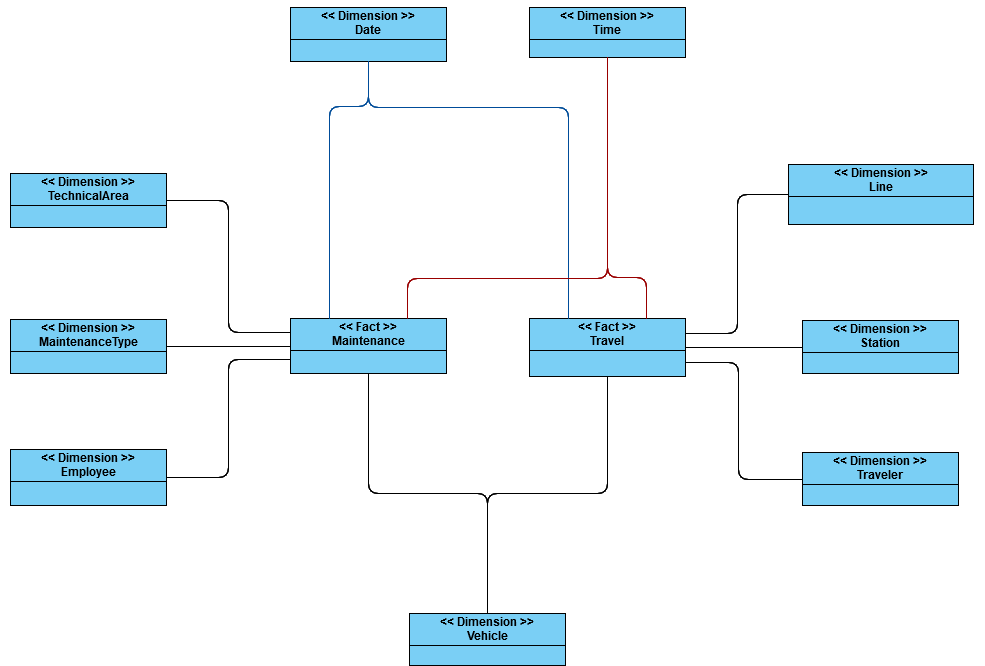
\includegraphics[scale=0.4]{images/data_warehouse.png}
  \caption{le \textit{data warehouse} résultant}
\end{figure}

\subsection{Estimation de la taille de l'entrepôt}
Dans notre entrepôt, on estime qu'on aura $365$ lignes pour la table \texttt{Date\_t} (\textit{i.e. le nombre de jours d'une année}) et 1440 lignes pour la table \texttt{Time\_t} (\textit{i.e. le nombre d'heures et minutes par jour}).

En outre, les estimations faites pour les autres tables sont basées sur des informations récoltées depuis les liens suivants :
\begin{itemize}
  \item \url{https://fr.wikipedia.org/wiki/Autobus_de_Montpellier}
  \item \url{https://www.verif.com/bilans-gratuits/TRANSPORTS-AGGLOMERATION-DE-MONTPELLIER-314871815/}
  \item \url{https://fr.wikipedia.org/wiki/Tramway_de_Montpellier}
  \item \url{https://e-metropolitain.fr/2016/12/17/une-visite-dans-les-coulisses-de-la-tam/}
  \item \url{http://taminst.tsi.cityway.fr/presentation/}
\end{itemize}

\begin{table}[!ht]
  \centering
  \begin{tabular}{|c|c|}
    \hline
    \textbf{Table} & \textbf{Taille}\\
    \hline
    \texttt{Date\_t} & $365$\\
    \hline
    \texttt{Time\_t} & $1440$\\
    \hline
    \texttt{Vehicle} & $270$\\
    \hline
    \texttt{Line} & $116$\\
    \hline
    \texttt{Station} & $654$\\
    \hline
    \texttt{TechnicalArea} & $2$\\
    \hline
    \texttt{MaintenanceType} & $\sim500$\\
    \hline
    \texttt{Employee} & $1144$\\
    \hline
  \end{tabular}
  \caption{taille estimée de chaque table de l'entrepôt}
\end{table}

\newpage

\chapter{Implémentation}
\section{Choix des technologies}
Afin d'implémenter notre entrepôt de données, nous avons décidé d'utiliser \texttt{Oracle}. De plus, pour chaque dimension partagée entre les deux \textit{data marts} nous avons créé deux vues virtuelles selon le niveau de détails nécessité pour l'analyse concernée.

\section{Requêtes analytiques du \textit{data-mart} des voyages}
Pour répondre à la problématique du \textit{data-mart} des voyages, nous avons effectué les requêtes analytiques suivantes\footnote{on affiche uniquement les premières lignes des résultats de chaque requête} :

\begin{lstlisting}[caption={le nombre de voyages par bus, utilisant des tickets pour le mois de juillet}, label={lst:requ1}]
  SELECT Travel.id_vehicle, COUNT(*) AS number_travel
  FROM Travel
  INNER JOIN Vehicle_travel ON Travel.id_vehicle = Vehicle_travel.id
  INNER JOIN Traveler ON Travel.id_traveler = Traveler.id
  INNER JOIN Date_travel ON Travel.id_date = Date_travel.id
  WHERE Vehicle_travel.type = 'bus'
  AND Traveler.anonymous = 1
  AND Date_travel.month_year = 7
  GROUP BY Travel.id_vehicle
  ORDER BY Travel.id_vehicle;
\end{lstlisting}

\begin{figure}[!ht]
  \centering
  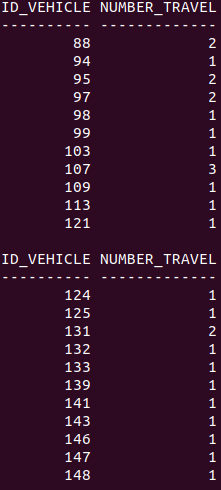
\includegraphics[scale=0.5]{images/requetes_analytiques/requ1.png}
  \caption{résultats de la requête \ref{lst:requ1}}
\end{figure}

\begin{lstlisting}[caption={le nombre de voyageurs abonnés par ligne pour chaque voyage pour les deux derniers mois}, label={lst:requ2}]
  SELECT Line.num_line, COUNT(Traveler.id) AS number_travelers
  FROM Travel
  INNER JOIN Line
    ON Travel.id_line = Line.id
  INNER JOIN Traveler
    ON Travel.id_traveler = Traveler.id
  INNER JOIN Date_travel
    ON Travel.id_date = Date_travel.id
  WHERE Date_travel.year = EXTRACT(YEAR FROM SYSDATE)
  AND Date_travel.month_year >= (EXTRACT(MONTH FROM SYSDATE) - 2)
  AND Traveler.anonymous = 0
  GROUP BY Line.num_line
  ORDER BY Line.num_line;
\end{lstlisting}

\begin{figure}[!ht]
  \centering
  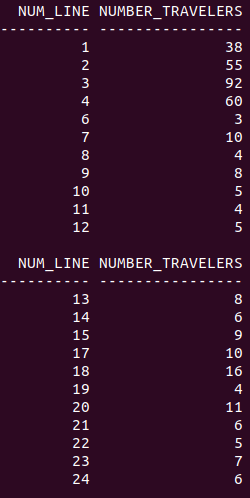
\includegraphics[scale=0.5]{images/requetes_analytiques/requ2.png}
  \caption{résultats de la requête \ref{lst:requ2}}
\end{figure}

\newpage

\begin{lstlisting}[caption={l'arrêt le plus fréquenté par ligne}, label={lst:requ3}]
  SELECT Line.num_line, Station.id, Station.name, COUNT(station.id) AS frequentation
  FROM Travel
  INNER JOIN Line
  	ON Travel.id_line = Line.id
  INNER JOIN Station
  	ON Travel.id_station = Station.id
  GROUP BY Line.num_line, Station.id, Station.name
  HAVING COUNT(Station.id) = (
    SELECT MAX(COUNT(*))
  	FROM Travel
  	INNER JOIN Line sl
  		ON Travel.id_line = sl.id
  	INNER JOIN Station
  		ON Travel.id_station = Station.id
  	WHERE sl.num_line = Line.num_line
  	GROUP BY Station.id)
  ORDER BY Line.num_line, Station.id;
\end{lstlisting}

\begin{figure}[!ht]
  \centering
  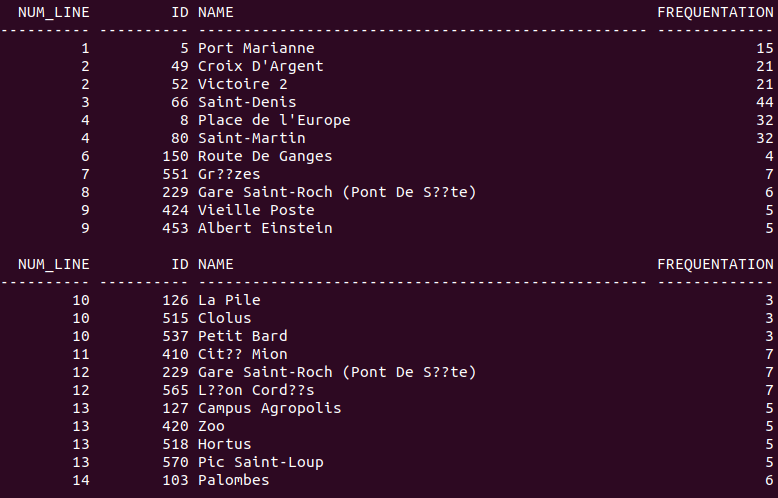
\includegraphics[scale=0.5]{images/requetes_analytiques/requ3.png}
  \caption{résultats de la requête \ref{lst:requ3}}
\end{figure}

\newpage

\begin{lstlisting}[caption={le nombre de voyages par heure pour chaque ligne}, label={lst:requ4}]
  SELECT Line.num_line, Time_travel.hours AS Hour, COUNT(*) AS number_travel
  FROM Travel
  INNER JOIN Line ON Travel.id_line = Line.id
  INNER JOIN Time_travel ON Travel.id_time = Time_travel.id
  GROUP BY Line.num_line, Time_travel.hours
  ORDER BY Line.num_line, Time_travel.hours;
\end{lstlisting}

\begin{figure}[!ht]
  \centering
  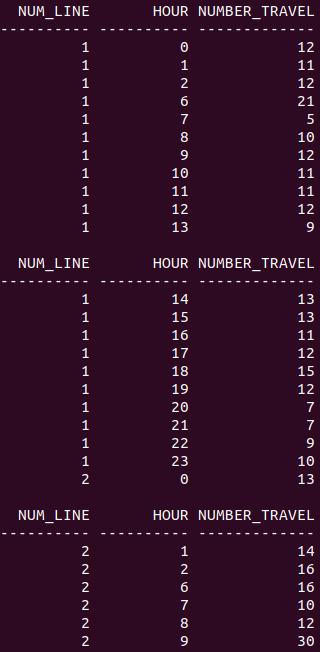
\includegraphics[scale=0.5]{images/requetes_analytiques/requ4.png}
  \caption{résultats de la requête \ref{lst:requ4}}
\end{figure}

\newpage

\begin{lstlisting}[caption={le véhicule le plus utilisé par les voyageurs par ligne}, label={lst:requ5}]
  SELECT Line.num_line, Vehicle_travel.id, COUNT(Vehicle_travel.id) AS number_vehicle
  FROM Travel
  INNER JOIN Line
    ON Travel.id_line = Line.id
  INNER JOIN Vehicle_travel
    ON Travel.id_vehicle = Vehicle_travel.id
  GROUP BY Line.num_line, Vehicle_travel.id
  HAVING COUNT(Vehicle_travel.id) = (
    SELECT MAX(COUNT(*))
    FROM Travel
    INNER JOIN Line sl
      ON Travel.id_line = sl.id
    INNER JOIN Vehicle_travel
      ON Travel.id_vehicle = Vehicle_travel.id
    WHERE sl.num_line = Line.num_line
    GROUP BY Vehicle_travel.id)
  ORDER BY Line.num_line, Vehicle_travel.id;
\end{lstlisting}

\begin{figure}[!ht]
  \centering
  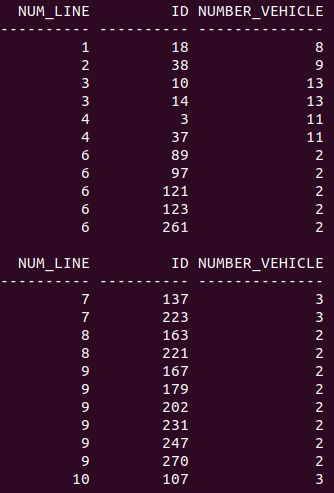
\includegraphics[scale=0.5]{images/requetes_analytiques/requ5.png}
  \caption{résultats de la requête \ref{lst:requ5}}
\end{figure}

\section{Requêtes analytiques du \textit{data-mart} des maintenances}
Pour répondre à la problématique du \textit{data-mart} des maintenances, nous avons effectué les requêtes analytiques suivantes :

\begin{lstlisting}[caption={le coût total de maintenance de chaque véhicule}, label={lst:requ6}]
  SELECT Vehicle_maintenance.id, SUM(cost)
  FROM Maintenance
  INNER JOIN Vehicle_maintenance
    ON Maintenance.id_vehicle = Vehicle_maintenance.id
  GROUP BY Vehicle_maintenance.id;
\end{lstlisting}

\begin{figure}[!ht]
  \centering
  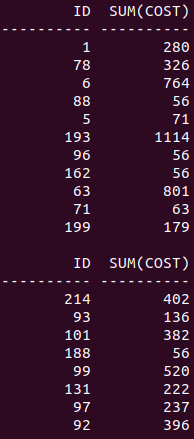
\includegraphics[scale=0.5]{images/requetes_analytiques/requ6.png}
  \caption{résultats de la requête \ref{lst:requ6}}
\end{figure}

\begin{lstlisting}[caption={le nombre total de maintenances effectuées sur les bus par employé pour l'année 2018}, label={lst:requ7}]
  SELECT Employee.id AS Employee, COUNT(*) as intervention
  FROM Maintenance
  INNER JOIN Employee
    ON Maintenance.id_employee = Employee.id
  INNER JOIN Vehicle_maintenance
    ON Maintenance.id_vehicle = Vehicle_maintenance.id
  INNER JOIN Date_maintenance
    ON Maintenance.id_date = Date_maintenance.id
  WHERE Vehicle_maintenance.type = 'bus'
  AND Date_maintenance.year = 2018
  GROUP BY Employee.id;
\end{lstlisting}

\begin{figure}[!ht]
  \centering
  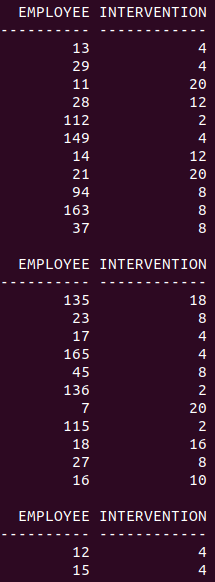
\includegraphics[scale=0.5]{images/requetes_analytiques/requ7.png}
  \caption{résultats de la requête \ref{lst:requ7}}
\end{figure}

\newpage

\begin{lstlisting}[caption={le nombre total de maintenances effectuées par véhicule pour les 6 dernier mois.}, label={lst:requ8}]
  SELECT Maintenance.id_vehicle, COUNT(*) AS number_maintenance
  FROM Maintenance
  INNER JOIN Vehicle_maintenance ON Maintenance.id_vehicle = Vehicle_maintenance.id
  INNER JOIN Date_maintenance ON Maintenance.id_date = Date_maintenance.id
  WHERE Date_maintenance.month_year >= (EXTRACT(MONTH FROM SYSDATE) - 6)
  AND Maintenance.id_operation_type = 5
  GROUP BY Maintenance.id_vehicle
  ORDER BY number_maintenance DESC;
\end{lstlisting}

\begin{figure}[!ht]
  \centering
  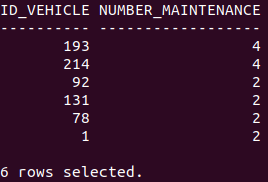
\includegraphics[scale=0.5]{images/requetes_analytiques/requ8.png}
  \caption{résultats de la requête \ref{lst:requ8}}
\end{figure}

\newpage

\begin{lstlisting}[caption={le type de maintenance le plus fréquent}, label={lst:requ9}]
  SELECT MaintenanceType.maintenance_type AS type, COUNT(Maintenance.id_maintenance_type) AS totalCount
  FROM Maintenance
  INNER JOIN MaintenanceType
    ON  MaintenanceType.id = Maintenance.id_maintenance_type
  GROUP BY MaintenanceType.maintenance_type
  HAVING COUNT(Maintenance.id_maintenance_type) = (
    SELECT MAX(COUNT(*))
    FROM Maintenance
    GROUP BY Maintenance.id_maintenance_type);
\end{lstlisting}

\begin{figure}[!ht]
  \centering
  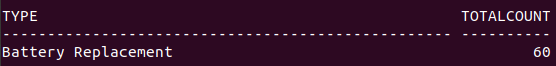
\includegraphics[scale=0.5]{images/requetes_analytiques/requ9.png}
  \caption{résultats de la requête \ref{lst:requ9}}
\end{figure}

\newpage

\begin{lstlisting}[caption={le nombre de maintenances par mois pour chaque local technique}, label={lst:requ10}]
  SELECT TechnicalArea.id, Date_maintenance.month_year, COUNT(Maintenance.id_technical_area) AS numberMaintenance
  FROM  Maintenance
  INNER JOIN  TechnicalArea
    ON Maintenance.id_technical_area = TechnicalArea.id
  INNER JOIN Date_maintenance
    ON Maintenance.id_date = Date_maintenance.id
  GROUP BY TechnicalArea.id, Date_maintenance.month_year
  ORDER BY TechnicalArea.id, Date_maintenance.month_year;
\end{lstlisting}

\begin{figure}[!ht]
  \centering
  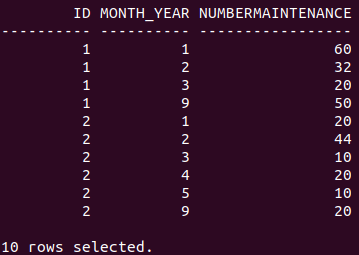
\includegraphics[scale=0.5]{images/requetes_analytiques/requ10.png}
  \caption{résultats de la requête \ref{lst:requ10}}
\end{figure}

\newpage

\begin{lstlisting}[caption={le nombre de véhicules maintenus le matin, et ceux maintenus l'après midi}, label={lst:requ11}]
  SELECT Time_maintenance.AM_PM_indicator, COUNT(Vehicle_maintenance.id) AS numberMaintenance
  FROM Maintenance
  INNER JOIN Vehicle_maintenance
    ON Maintenance.id_vehicle = Vehicle_maintenance.id
  INNER JOIN Time_maintenance
    ON Maintenance.id_time = Time_maintenance.id
  GROUP BY Time_maintenance.AM_PM_indicator;
\end{lstlisting}

\begin{figure}[!ht]
  \centering
  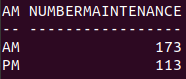
\includegraphics[scale=0.5]{images/requetes_analytiques/requ11.png}
  \caption{résultats de la requête \ref{lst:requ11}}
\end{figure}

\chapter{Conclusion}
\section{Plan}
Dans ce modèle nous avons proposé un outil permettant d'effectuer des analyses afin de repondre à des problématiques précises et bien définies.
Pour ce faire, analyser chaque voyage s'est avéré essentiel. En effet, l'objectif principal de \textit{tam-voyages} est de maximiser le nombre de voyages effectués dans son réseau et d'améliorer sa qualité de service. Il était donc logique de prioriser l'analyse des voyages effectués selon les voyageurs et titre de transport (ticket, abonnement) utilisés.

D'autre part, nous avons réalisé un outil répondant à des questions pertinentes à la problématique secondaire. Par conséquent, nous avons proposé d'analyser les différentes transactions effectuées lors des maintenances des véhicules.

En conclusion, notre modèle répond bien à un ensemble de questions primordiales par rapport aux objectifs de \textit{tam-voyages}.

\section{Perspectives}
Bien que, notre modèle nous a permis de réaliser des analyses indispensables, nous avons constaté qu'il était assez limité. Effectivement, il est incapable de calculer le montant exact du chiffre d'affaires de \textit{tam-voyages} en termes de ventes de tickets et de frais d'abonnements. Par ailleurs, on ne peut pas connaître la fréquentation de chaque trajet effectué par un véhicule; on peut uniquement connaître les arrêts.

Par suite, des perspectives d'évolution de l'entrepôt sont possibles.

\subsection{\textit{Data Marts} pour la vente des tickets et les abonnements}
Afin de pallier le probléme de la vente des tickets et les abonnements, nous proposons la perspective d'évolution suivante :
\begin{enumerate}
  \item l'ajout d'un \textit{Data mart} ayant comme action la vente d'un ticket à un voyageur à une date donnée avec une mesure désignant le prix du ticket vendu
  \item l'ajout d'un \textit{Data mart} ayant comme action l'abonnement d'un voyageur à une date donnée avec des mesures désignant les frais de l'abonnement et sa durée de validité
\end{enumerate}

Ainsi, l'analyse des bénéfices recoltées à travers ces deux actions permet, entre autres, d'approximer le chiffre d'affaires de \textit{tam-voyages}\footnote{on ne compte pas les bénéfices récoltées via d'autres moyens tels que \textit{VéloMagg} ou d'autres}.

\subsection{\textit{Data Mart} pour les trajets effectués par des véhicules}
Afin de pallier le problème de fréquentation de chaque trajet effectué par un véhicule, nous proposons la perspective suivante :
\begin{enumerate}
  \item l'ajout d'un \textit{Data Mart} tel que chaque fait soit désigné par un trajet effectué par un véhicule sur une ligne du réseau de transport à une date et une heure donnée, sans aucune mesure à expliciter.
  \item l'idée dans cette vision consiste à modifier la table des voyages (développée auparavant) pour raffiner les analyses de manière à inclure des informations supplémentaires sur les trajets, non incluses dans la version initiale proposée.
  \item un fait dans ladite table désignera ainsi un voyage effectué par un voyageur dans un véhicule faisant un trajet sur une ligne du réseau de transport à une date et une heure donnée.
  \item pour ce faire, il faut lier la table des voyages avec la table des trajets (i.e. rajouter un attribut \textbf{id\_trajet} dans la table \texttt{Travel}).
\end{enumerate}

Ainsi, cette solution nous permettra de raffiner le grain d'analyse d'un voyage en incluant le trajet effectué par le véhicule concerné.

\end{document}
